%%%%%%%%%%%%%%%%%%%%%%%%%%%%%%%%%%%%%%%%%
% Beamer Presentation
% LaTeX Template
% Version 1.0 (10/11/12)
%
% This template has been downloaded from:
% http://www.LaTeXTemplates.com
%
% License:
% CC BY-NC-SA 3.0 (http://creativecommons.org/licenses/by-nc-sa/3.0/)
%
%%%%%%%%%%%%%%%%%%%%%%%%%%%%%%%%%%%%%%%%%

%----------------------------------------------------------------------------------------
%	PACKAGES AND THEMES
%----------------------------------------------------------------------------------------

\documentclass{beamer}

\mode<presentation> {

% The Beamer class comes with a number of default slide themes
% which change the colors and layouts of slides. Below this is a list
% of all the themes, uncomment each in turn to see what they look like.

%\usetheme{default}
%\usetheme{AnnArbor}
%\usetheme{Antibes}
%\usetheme{Bergen}
%\usetheme{Berkeley}
%\usetheme{Berlin}
%\usetheme{Boadilla}
%\usetheme{CambridgeUS}
%\usetheme{Copenhagen}
%\usetheme{Darmstadt}
%\usetheme{Dresden}
%\usetheme{Frankfurt}
%\usetheme{Goettingen}
%\usetheme{Hannover}
%\usetheme{Ilmenau}
%\usetheme{JuanLesPins}
%\usetheme{Luebeck}
\usetheme{Madrid}
%\usetheme{Malmoe}
%\usetheme{Marburg}
%\usetheme{Montpellier}
%\usetheme{PaloAlto}
%\usetheme{Pittsburgh}
%\usetheme{Rochester}
%\usetheme{Singapore}
%\usetheme{Szeged}
%\usetheme{Warsaw}

% As well as themes, the Beamer class has a number of color themes
% for any slide theme. Uncomment each of these in turn to see how it
% changes the colors of your current slide theme.

%\usecolortheme{albatross}
%\usecolortheme{beaver}
%\usecolortheme{beetle}
%\usecolortheme{crane}
%\usecolortheme{dolphin}
%\usecolortheme{dove}
%\usecolortheme{fly}
%\usecolortheme{lily}
%\usecolortheme{orchid}
%\usecolortheme{rose}
%\usecolortheme{seagull}
%\usecolortheme{seahorse}
%\usecolortheme{whale}
%\usecolortheme{wolverine}

%\setbeamertemplate{footline} % To remove the footer line in all slides uncomment this line
%\setbeamertemplate{footline}[page number] % To replace the footer line in all slides with a simple slide count uncomment this line

%\setbeamertemplate{navigation symbols}{} % To remove the navigation symbols from the bottom of all slides uncomment this line
}
\usepackage{romannum}
\usepackage{setspace}
\usepackage{tipa}
\usepackage{graphicx} % Allows including images
\usepackage{booktabs} % Allows the use of \toprule, \midrule and \bottomrule in tables

%----------------------------------------------------------------------------------------
%	TITLE PAGE
%----------------------------------------------------------------------------------------

\title[Dissertation Proposal]{ Weighing Segmental/Syllable Errors in Foreign Accent} % The short title appears at the bottom of every slide, the full title is only on the title page

\author{Zhiyan Gao \& Steven Weinberger} % Your name
\institute[GMU] % Your institution as it will appear on the bottom of every slide, may be shorthand to save space
{
George Mason University \\ % Your institution for the title page
\medskip
\textit{Accents 2017} % Your email address
}
\date{Dec.2 2017} % Date, can be changed to a custom date




\begin{document}

\begin{frame}
\titlepage % Print the title page as the first slide
%\textsubscript{Committee:}\linebreak
%\textsubscript{Steven Weinberger, PhD}\linebreak
%\textsubscript{Douglas Wulf, PhD}\linebreak
%\textsubscript{Dennis Perzanowski, PhD}
\end{frame}

%\begin{frame}
%\frametitle{Overview} % Table of contents slide, comment this block out to remove it
%\tableofcontents % Throughout your presentation, if you choose to use \section{} and \subsection{} commands, these will automatically be printed on this slide as an overview of your presentation
%\end{frame}

%----------------------------------------------------------------------------------------
%	PRESENTATION SLIDES
%----------------------------------------------------------------------------------------

%------------------------------------------------
\section{Introduction}
\begin{frame}
\frametitle{Introduction}
\begin{enumerate}
\onslide<1->{\item {\bf Foreign Accent}}\linebreak\linebreak
\onslide <2->\textit{Adult learners' L2 speech is often perceived as accented\linebreak\textsubscript{(Flege, Munro, \& Mackay, 1995)}}\linebreak
\linebreak
\onslide<3->\textit{The {\bf perceivable} deviation of non-native speech from the native speech norm is often defined as “foreign accent”.\linebreak\textsubscript {(Munro \& Derwing, 1998)} }\linebreak
\linebreak
\onslide<4->{\item {\bf Accentedness Perception}}\linebreak\linebreak
\onslide<5->\textit{Native speakers can detect foreign accent even in very short L2 speech samples}\linebreak\textsubscript{30ms-long stimuli (Flege,1984), ERP N100 (Steinschneider et. al., 1999)}
\end{enumerate}
\end{frame}

\section{Research Questions} % Sections can be created in order to organize your presentation into discrete blocks, all sections and subsections are automatically printed in the table of contents as an overview of the talk
%------------------------------------------------

%\subsection{Subsection Example} % A subsection can be created just before a set of slides with a common theme to further break down your presentation into chunks
\begin{frame}
\frametitle{Research Questions}
\begin{spacing}{2}
\begin{enumerate}
\onslide<1->{\item What are the segmental/structural attributes of {\bf foreign accent}?}
\onslide<2->{\item Do some L2 speech errors contribute more to accent than others?}
%\onslide<3->{\item Why some L2 errors are more accented than others?}
\end{enumerate}
\end{spacing}
\end{frame}

\section{Background}
\subsection{L2 errors that affects accentedness}
\begin{frame}
\frametitle{Background \Romannum{1}:L2 Errors}
\begin{itemize}
\onslide<1->{\item Consonant errors affects accentedness \linebreak
\textit{VOT, Liquids \linebreak \textsubscript{(Gonzalez-Bueno,1997; Solon,2015)}}\linebreak}
\onslide<2->{\item Vowels are complicated \linebreak
\textit{Duration, Formats, Vowel space \textsubscript{(Major, 1987;McCullough,2013;Chan, Hall, and Assgari,2016)}}\linebreak}
\onslide<3->{\item What about syllables?\linebreak
\textit{Segment Insertion, Segment Deletion \linebreak\textsubscript{(Magen, 1998; Van Doel, 2006)}}}
\end{itemize}
\end{frame}


\subsection{The degree of accentedness}
%Magen(1998)
\begin{frame}
\frametitle{Background \Romannum{2}: the Ranking of Errors}
\onslide<1->{\begin{block}{Magen (1998):speaker 1}
Epenthetic schwa, -ed ending, {\bf tense-lax}, final/s/, \textipa{tS} to \textipa{S}, lexical and phrasal stress\linebreak  $>>$ \linebreak\
Stop voicing,/s/ to /z/, vowel reduction 
\end{block}
}
\onslide<2->{\begin{block}{Magen (1998):speaker 2}
Epenthetic schwa, final/s/, \textipa{tS} to \textipa{S}, lexical and phrasal stress\linebreak  $>>$ \linebreak
Stop voicing,/s/ to /z/, vowel reduction, {\bf tense-lax}
\end{block}
}
\begin{itemize}
\onslide<3->{\item Errors were artificially added}
\onslide<4->{\item Each stimulus may contain more than 1 error}
\onslide<5->{\item F0 contours were synthesized}
\onslide<6->{\item Types of errors were limited}
\end{itemize}
\end{frame}
%Doel(2006)
\begin{frame}
\frametitle{Background \Romannum{2}: the Ranking of Errors}
\onslide<1->{\begin{block}{van Doel (2006)}
Lexical Stress, Uvular-r $>>$ \linebreak\linebreak
Voicing, Epenthesis in /lm/, /w/ to /v/, /\textipa{\ae}/ to /e/ $>>$ \linebreak\linebreak
Coda weakening in "off" and "that" $>>$ \linebreak\linebreak
VOT shortening on /t\super h/,/\textipa{2}/ to /\textipa{A}/,intonation $>>$ \linebreak\linebreak
yod-insertion in "news"
\end{block}
}
\begin{itemize}
\onslide<2->{\item Stimuli were produced by native speakers}
\onslide<3->{\item Not fair to compare "vine (L1:wine)" to "dell (L1:tell)"}
\onslide<4->{\item Problems with prosody cloning}
\onslide<5->{\item 5-point rating scale is inadequate}
\end{itemize}
\end{frame}
%Gao(2016)
\begin{frame}
\frametitle{Background \Romannum{2}: the Ranking of Errors}
\only <1>{
\begin{block}{Gao (2016): Consonant$>>$Syllable$>>$Vowel}
\begin{figure}
\includegraphics[width=0.7\linewidth]{barchart}
\end{figure}
\end{block}}
\only <2>{
\begin{block}{Gao (2016):The trend does not always hold}
\begin{figure}
\includegraphics[width=0.8\linewidth]{ft_detailed}
\end{figure}
\end{block}}

\end{frame}
%------------------------------------------------------------------------
\subsection{Why L2 errors exhibit various degree of accentedness}
\begin{frame}
\frametitle{Background \Romannum{3}: \linebreak Why some L2 errors are more/less accented?}
\onslide<1->{What did previous studies say?}
\begin{enumerate}
\onslide<2->{\item Native speech has the same type of "errors". \linebreak 
	(e.g. /d/ to /t/, /\textipa{T}/ to /t/) \linebreak}
\onslide<3->{\item Some sounds don't exist in English, which {\bf could} be more salient. \linebreak
	(e.g. /s/ to /\textipa{\:s}/) \linebreak}
\onslide<4->{\item Some L2 errors defy English phonotactics.\linebreak
	(e.g. /b\textipa{E}t/ to /b\textipa{E}/)\linebreak-- a monosyllabic content word should contain at least two moras). \linebreak}
\onslide<5->{\item Consonant errors are inherently more salient than vowel errors,\linebreak due to the divide between
	{\bf categorical} and {\bf episodic perception}.}
\end{enumerate}
\end{frame}
%---------------------------------------------------
\begin{frame}
\frametitle{Background \Romannum{3}: \linebreak Why some L2 errors are more/less accented?}
\onslide<1->{Proposal: \linebreak\linebreak
Accentedness of an L2 speech pattern depends on\linebreak}
\begin{enumerate}
\onslide<2->{\item How likely it exists in native English speech\linebreak
e.g. How likely "bob" becomes "bop" in native speech\linebreak}
\onslide<3->{\item How well-formed it is, in terms of feature bundles \linebreak
	e.g. /s/ to /\textipa{\:s}/ --$>$ *[+word initial, +retroflex] \linebreak
	e.g. /b\textipa{E}t/ to /b\textipa{E}/--$>$ *[+lax,+word final]. \linebreak}
\onslide<4->{\item Is it vowel-related or consonant-related}
\end{enumerate}
\end{frame}
%-------------------------------------------
\section{The Current Study}
\subsection{overview}
\begin{frame}
\frametitle{The current study \Romannum{1}: Aims}
\begin{enumerate}
\item{Design a perception study to obtain accentedness ratings;}\linebreak
\item{Rank the L2 errors by accentedness;}\linebreak
\item{Adopt a Bayesian approach to show accentedness relates to well-formedness;}\linebreak
\end{enumerate}
\end{frame}

%------------------------------------------------
\subsection{Research design}
\begin{frame}
\frametitle{The current study \Romannum{1}: Research Design}
Stimuli:
\begin{itemize} 
\item 1 error per stimulus
\item compare errors in the same environment
\item no prosody manipulation 
\end{itemize}
\begin{table}
\begin{tabular}{lllll}
\toprule
& \textbf{consonant} & \textbf{vowel} & \textbf{syllable} & \textbf{correct} \\
\midrule
please call   & /\textipa{\underline{\color{red}b}li:z k\super hAl/ } & /\textipa{p\super hli:z k\super h\underline{\color{red}o}l/}&/\textipa{p\super h\underline{\color{red}@}li:z k\super hAl/} &/\textipa{p\super hli:z k\super hAl/}  \\ 
ask her       &/\textipa{\ae sk (h)@\underline{\color{red}r}}/            &/\textipa{\underline{\color{red}A}sk (h)@\*r}/        &/\textipa{\ae s\underline{ } h@\*r}/           &/\textipa{\ae sk (h)@\*r}/      \\
six spoons    &\textipa{/sIks spun\underline{\color{red}S}/ }             &\textipa{/s\underline{\color{red}i}ks spunz/ }         &\textipa{/sIks \underline{\color{red}@}spunz/ }            &\textipa{/sIks spunz/ }        \\
five thick    &/\textipa{faIv \underline{\color{red}t}Ik}/            &/\textipa{f\underline{\color{red}a }v TIk}/        & /\textipa{faIv\underline{\color{red}@} TIk}/          & /\textipa{faIv TIk}/        \\
small plastic &/\textipa{smO\underline{\color{red}\:l}}           &/\textipa{smOl}         &/\textipa{smOl}           &/\textipa{smOl}\\
	&\textipa{p\super hl\ae stIk}	&\textipa{p\super hl\ae st\underline{\color{red}i}k}	& \textipa{p\super hl\ae s\underline{ }Ik}/	&\textipa{p\super hl\ae stIk}/  \\
\bottomrule  
\end{tabular}
\end{table}
\end{frame}
%------------------------------------------------
\begin{frame}
\frametitle{The current study \Romannum{1}: Research Design}
Stimuli collection: \linebreak
natural speech sample from the Speech Accent Achieve via \textbf{crowd-sourced} transcriptions 
\begin{columns}[c] % The "c" option specifies centered vertical alignment while the "t" option is used for top vertical alignment
\column{.5\textwidth} % Left column and width
\begin{figure}
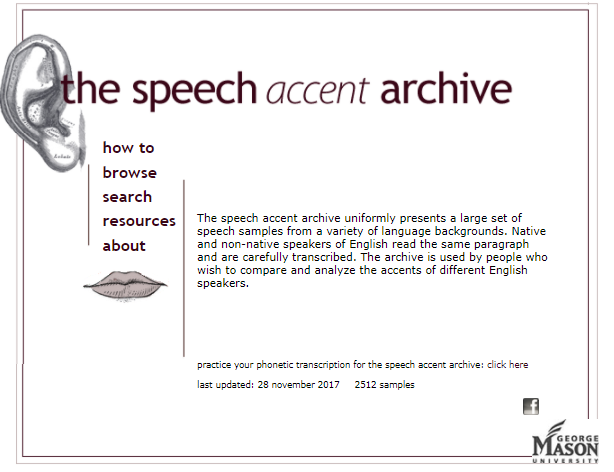
\includegraphics[width=0.8\linewidth]{accent}
\linebreak \textsubscript{accent.gmu.edu}
\end{figure}
\column{.5\textwidth} % Right column and width
\begin{figure}
\includegraphics[width=0.8\linewidth]{trans}
\linebreak \textsubscript{transcriber.accent.gmu.edu}
\end{figure}
\end{columns}
\end{frame}
%-----------------------------------------------
\subsection{Rationale}
\begin{frame}
\frametitle{The current study \Romannum{1}: Research Design}
Rationale/Advantages of the design:
\begin{spacing}{2}
\begin{itemize}
\onslide<1->{
\item Stimuli will be representative of L2 speech }
\onslide<2->{
\item L2 errors will be determined by hundreds if not thousands of people
\begin{itemize}
\item No need to "construct" errors
\end{itemize}}
\onslide<3->{
\item Phonological environment is controlled}
\onslide<4->{
\item Plenty of native English data as control}
\onslide<5->{
\item No prosody manipulation}
\end{itemize}
\end{spacing}
\end{frame}

%------------------------------------------------
\subsection{Interface}
\begin{frame}
\frametitle{The current study \Romannum{1}: Research Design}
\begin{itemize}
\item Platform: Amazon Mechanical Turk 
\item Participants: 100 native English speakers
\item Procesure: 20 stimuli for training, 80 stimuli for testing
\item Interface:
\end{itemize}
\begin{figure}
\includegraphics[width=0.7\linewidth]{demo}
\linebreak \textsubscript{Demo at http://mason.gmu.edu/\~{}zgao/mturk}
\end{figure}
\end{frame}

%------------------------------------------------

%------------------
\subsection{Data Analysis}

\begin{frame}
\frametitle{The current study \Romannum{2}: Data Analysis}
Prosody Control: Dynamic Time Warping (DTW) 
\begin{itemize}
\item No acoustic manipulation required
\item Align F0 contours of two utterances
\item Produce a DTW score which represents alignment cost
\item Bigger the DTW score, bigger the intonational difference
\end{itemize}
\begin{columns}[c] % The "c" option specifies centered vertical alignment while the "t" option is used for top vertical alignment
\column{.45\textwidth} % Left column and width
\begin{figure}
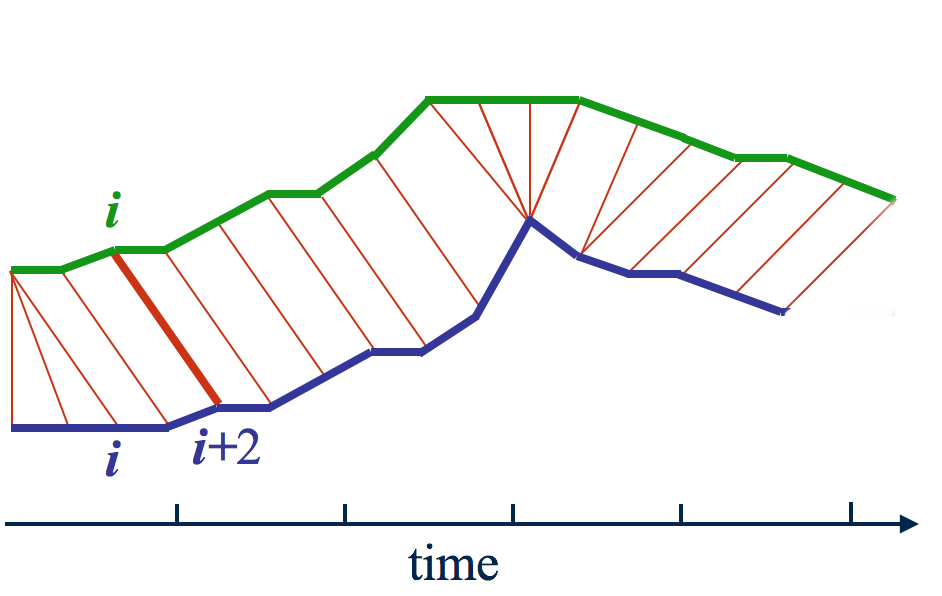
\includegraphics[width=0.8\linewidth]{dtw1}
\linebreak \textsubscript{(Tsiporkova, 2007) }
\end{figure}
\column{.55\textwidth} % Right column and width
\begin{figure}
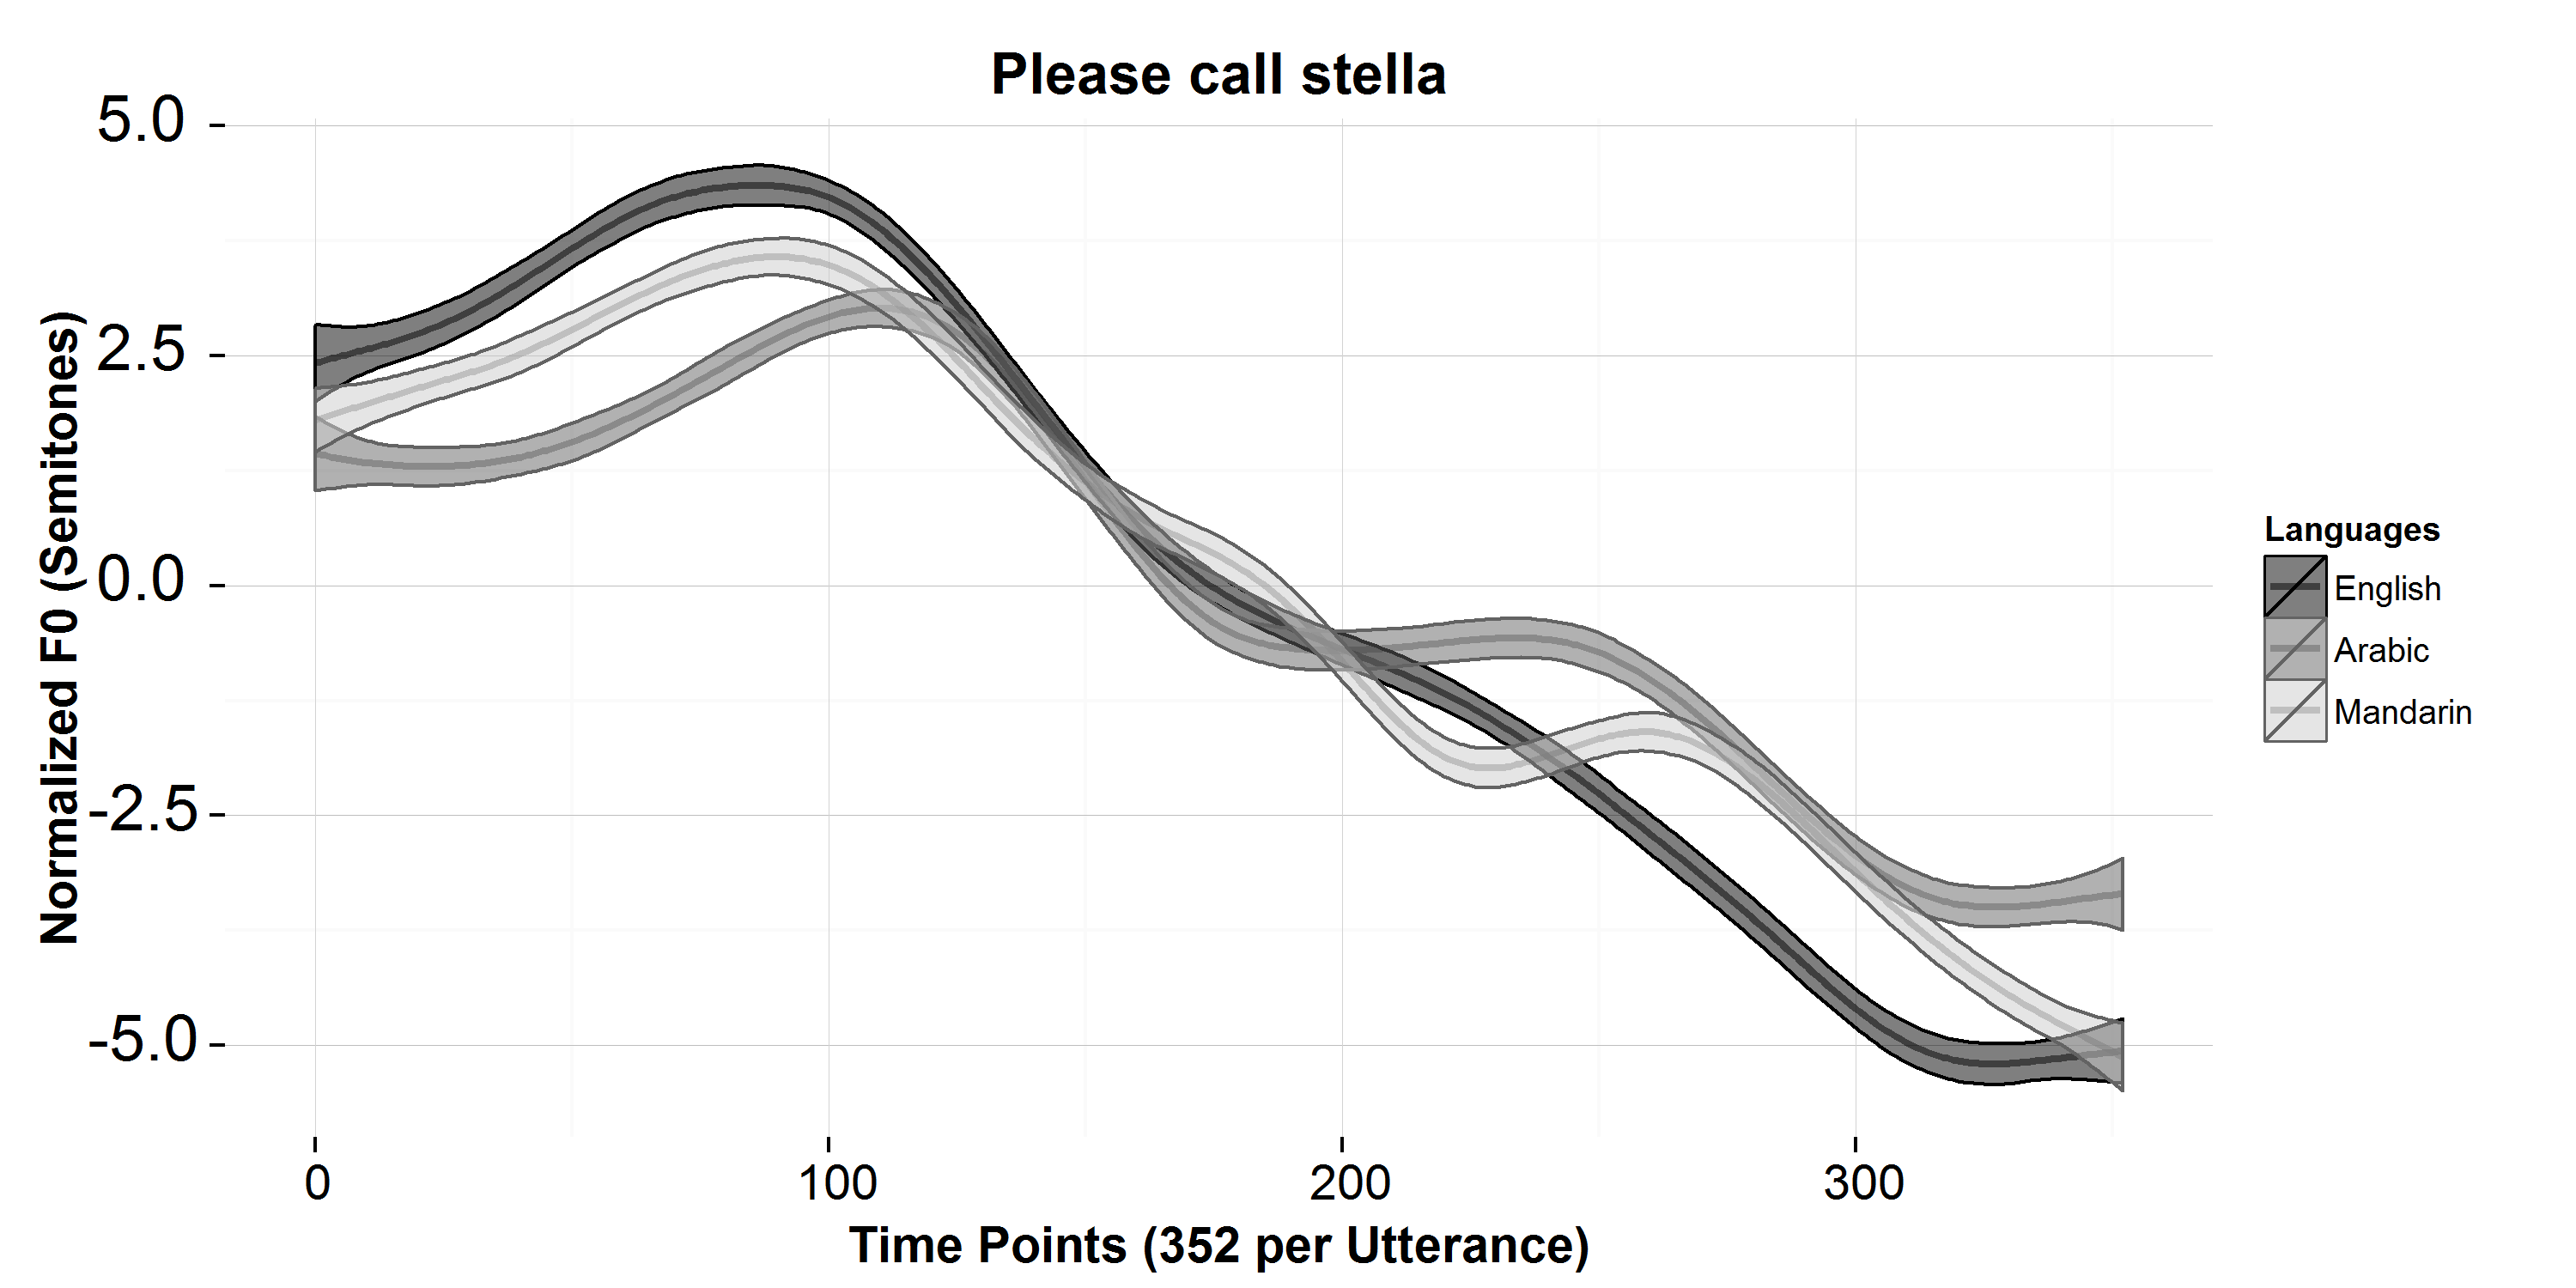
\includegraphics[width=0.9\linewidth]{dtw2}
\linebreak\textsubscript{(Morrill \& Gao,2016)}
\end{figure}
\end{columns}
\end{frame}

%------------------------------------------------

\begin{frame}
\frametitle{The current study \Romannum{2}: Data Analysis}
\onslide<1->{Obtain measurements for
\begin{itemize}
\item How likely an L2 speech pattern exist in native English speech
\item How well-formed an L2 speech pattern is\linebreak
\end{itemize}}
\onslide<2->{A Bayesian interpretation\textsubscript{(Wilson \& Davidson, 2013)}\linebreak
e.g. "please" --$>$ "blease" \linebreak
\begin{itemize}
\item The likelihood for a native-like "p" to exhibit acoustic features of the "b" --\textit{\bf the likelihood function}
\begin{itemize}
\item[] {Given VOT of /p/ (M=67,SD=22), if VOT of /b/=10, then Pr(b\big|p)=0.005}\linebreak
\end{itemize}
\onslide<3->{\item How well-formed "blease" is -- \textit{\bf the prior}
\begin{equation}
\Pr(/b/|/p/) \propto exp( \beta \cdot /p/acoustics) \cdot \text{Well-formedness of /bl/}
\end{equation}}
\end{itemize}}
\end{frame}
%------------------------------------------------
%-----------------------------------------------
\subsection{MaxEnt}
\begin{frame}
\frametitle{The current study \Romannum{2}: Data Analysis}
Maximum Entropy as Well-formedness \textsubscript{(Hayes \& Wilson, 2008)}\linebreak
\begin{table}[]
\caption{Pilot study-- Well-formedness of Mandarin accent}
\label{my-label}
\begin{tabular}{lllll}
\toprule
       & \textsubscript{\bf *{[}+continuant{]}{[}+voice,-coronal{]} }&....&  \textsubscript{\bf *{[}+voice{]}{[}-coronal{]}} & MaxEnt \\
 \midrule
sm  &      \multicolumn{1}{c}{0.179}            &  ...          &  \multicolumn{1}{c}{0}   &  \multicolumn{1}{c}{1.619}      \\
\textipa{S}m & \multicolumn{1}{c}{0.179}          & ...           &\multicolumn{1}{c}{0}       & \multicolumn{1}{c}{\color{red}10.648}       \\
\textipa{\:s}m & \multicolumn{1}{c}{0.179}          & ...           &\multicolumn{1}{c}{0}       & \multicolumn{1}{c}{\color{red}11.224}       \\
\textipa{C}m &       \multicolumn{1}{c}{0.179}   & ...           & \multicolumn{1}{c}{0}      & \multicolumn{1}{c}{\color{red}11.712}     \\
zm & \multicolumn{1}{c}{0.179}	&...	&\multicolumn{1}{c}{1.021}	&\multicolumn{1}{c}{\color{red}13.893}	\\
\bottomrule
\end{tabular}
\end{table}
\textsubscript{L2 data: GMU Speech Accent Archive}\linebreak
\textsubscript{English data: CMU Sphinx Dictionary}
\end{frame}

%------------------------------------------------
\subsection{Predictions}
\begin{frame}
\frametitle{The current study \Romannum{3}: Predictions}
\begin{block}{Ranking of Errors}
\begin{figure}
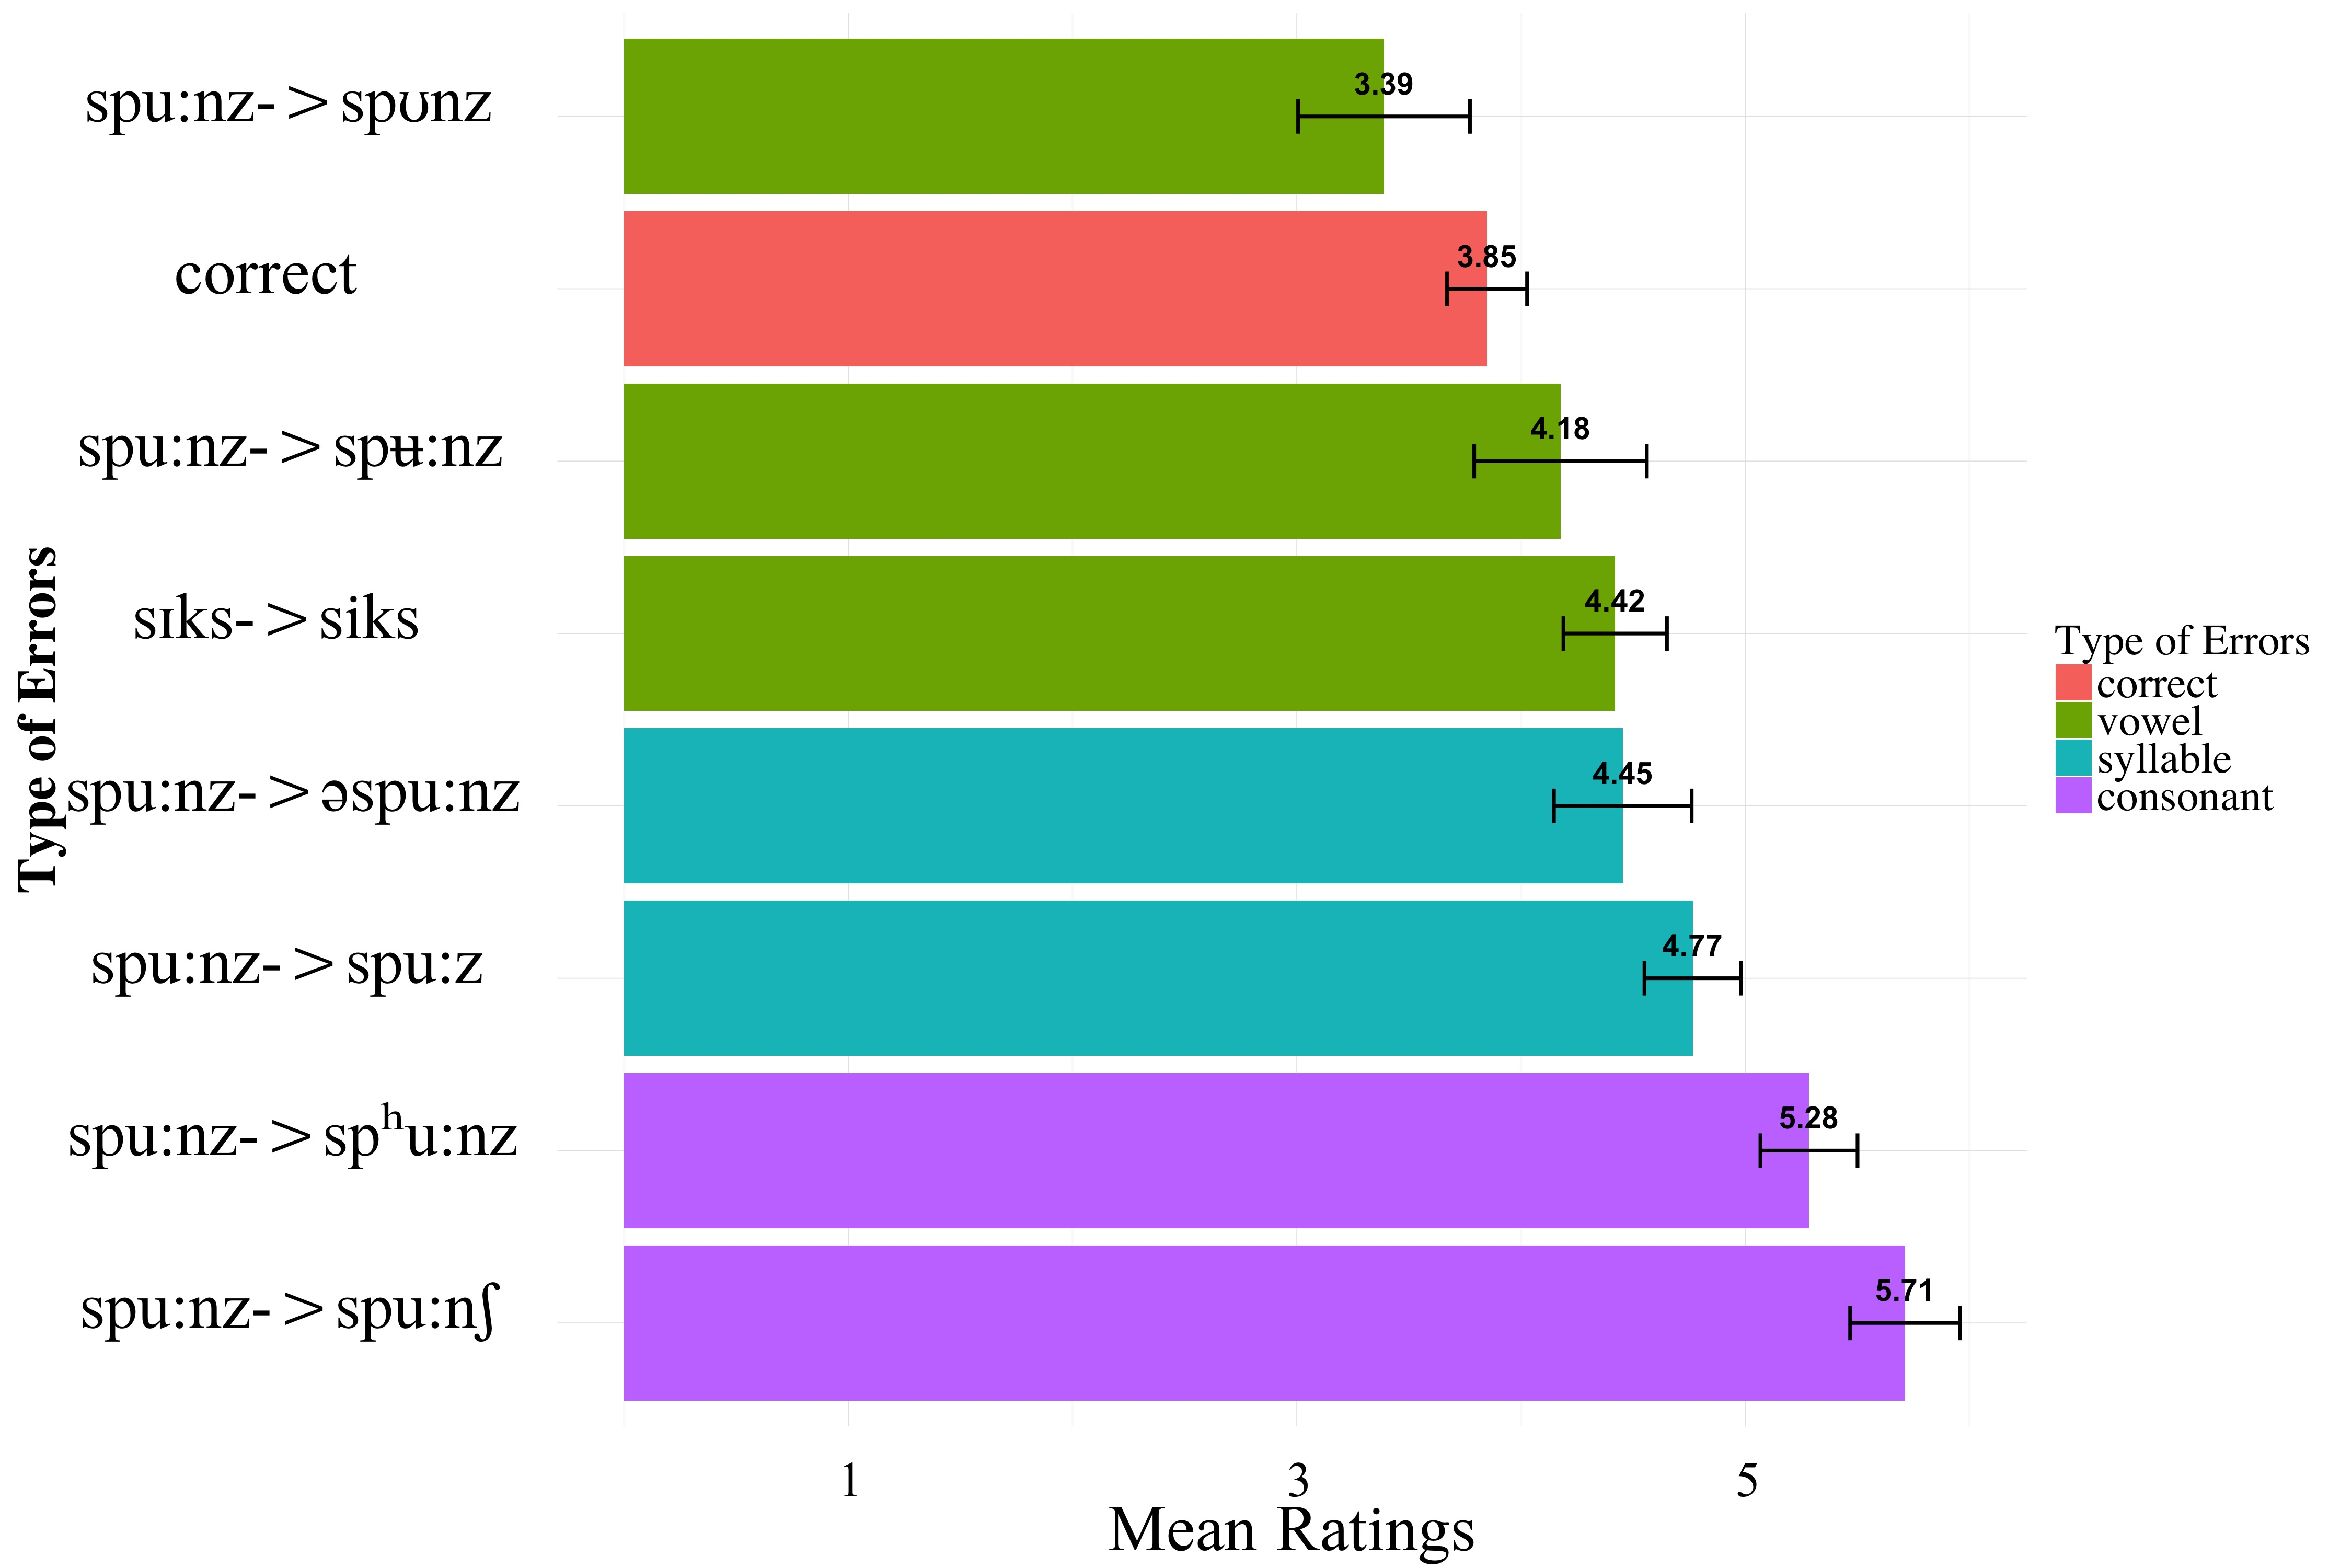
\includegraphics[width=0.8\linewidth]{ss_detailed}
\end{figure}
\end{block}
\end{frame}
\begin{frame}
\frametitle{The current study \Romannum{3}: Predictions}
\begin{block}{Well-formedness \& Accentedness}
\begin{figure}
\includegraphics[width=0.8\linewidth]{red}
\end{figure}
\end{block}
\end{frame}
%------------------------------------------------

%------------------------------------------------


%------------------------------------------------
\section{Timeline}
\begin{frame}
\begin{block}{Timeline}
\begin{itemize}
\item May 1 to June 30: \linebreak the second behavioral study (pilot)
\item July 1 to August 31: 
\begin{itemize}
\item Bayesian modeling
\item Submit a draft to the 11th International Conference on Native and Non-native Accents of English (University of \L{}\'{o}d\'{z},
 Poland)
\end{itemize}
\item September 1 to November 30:
\begin{itemize}
\item the second behavioral study with new transcription data from Professor Weinberger's crowed-sourced project.
\item start writing the dissertation 
\end{itemize}
\item Spring 2018: Finish the dissertation and defend it. 
\end{itemize}
\end{block}
\end{frame}
%------------------------------------------------
\section{References}
\begin{frame}[shrink=20]
\frametitle{References}
\footnotesize{
\begin{itemize}
\item Chan, K. Y., Hall, M. D., \& Assgari, A. A. (2016). The role of vowel formant frequencies and duration in the perception of foreign accent. \emph {Journal of Cognitive Psychology}, 1\textendash{}12.
\item Hayes, B., \& Wilson, C. (2008). A maximum entropy model of phonotactics and phonotactic learning. \emph{Linguistic inquiry}, 39(3), 379-440.
\item Magen, H. S. (1998). The perception of foreign-accented speech. \emph{Journal of Phonetics}, 26(4), 381\textendash{}400.
\item Major, R. C. (1987). Phonological similarity, markedness, and rate of L2 acquisition. \emph{Studies in Second Language Acquisition}, 9(01), 63\textendash{}82.
\item Morrill, T., \& Gao, Z. (2016). Discriminability of non-native tonal contours in low-pass filtered speech. \emph{The Journal of the Acoustical Society of America}, 139(4), 2162-2163.
\item McCullough, E. A. (2013). \emph{Acoustic correlates of perceived foreign accent in non-native English}. The Ohio State University (Doctorate Dissertation). 
\item Solon, M. (2015). L2 Spanish/l: The Roles of F2 and Segmental Duration in Foreign Accent Perception. \emph{In Selected Proceedings of the 6th Conference on Laboratory Approaches to Romance Phonology} (pp. 83\textendash{}94). 
\item Van den Doel, R. (2006). \emph{How friendly are the natives? An evaluation of native-speaker judgements of foreign-accented British and American English }(Doctoral dissertation, Netherlands Graduate School of Linguistics).
\item Weinberger, S. H. (2016). \emph{Speech accent archive }[Database]. Retrieved from http://accent.gmu.edu
\item Wilson, C., \& Davidson, L. (2013). Bayesian analysis of non-native cluster production. \emph{In Proceedings of NELS (Vol. 40).} 


\end{itemize}}
\end{frame}

%------------------------------------------------

\begin{frame}
\Huge{\centerline{Thank You!}}
\end{frame}

%----------------------------------------------------------------------------------------
\section{Supplemental Materials}
\subsection{Ratings}
\begin{frame}
\frametitle{Supplemental Materials \Romannum{1}: Ratings}
\only <1>{
\begin{block}{Gao (2016):The trend does not always hold}
\begin{figure}
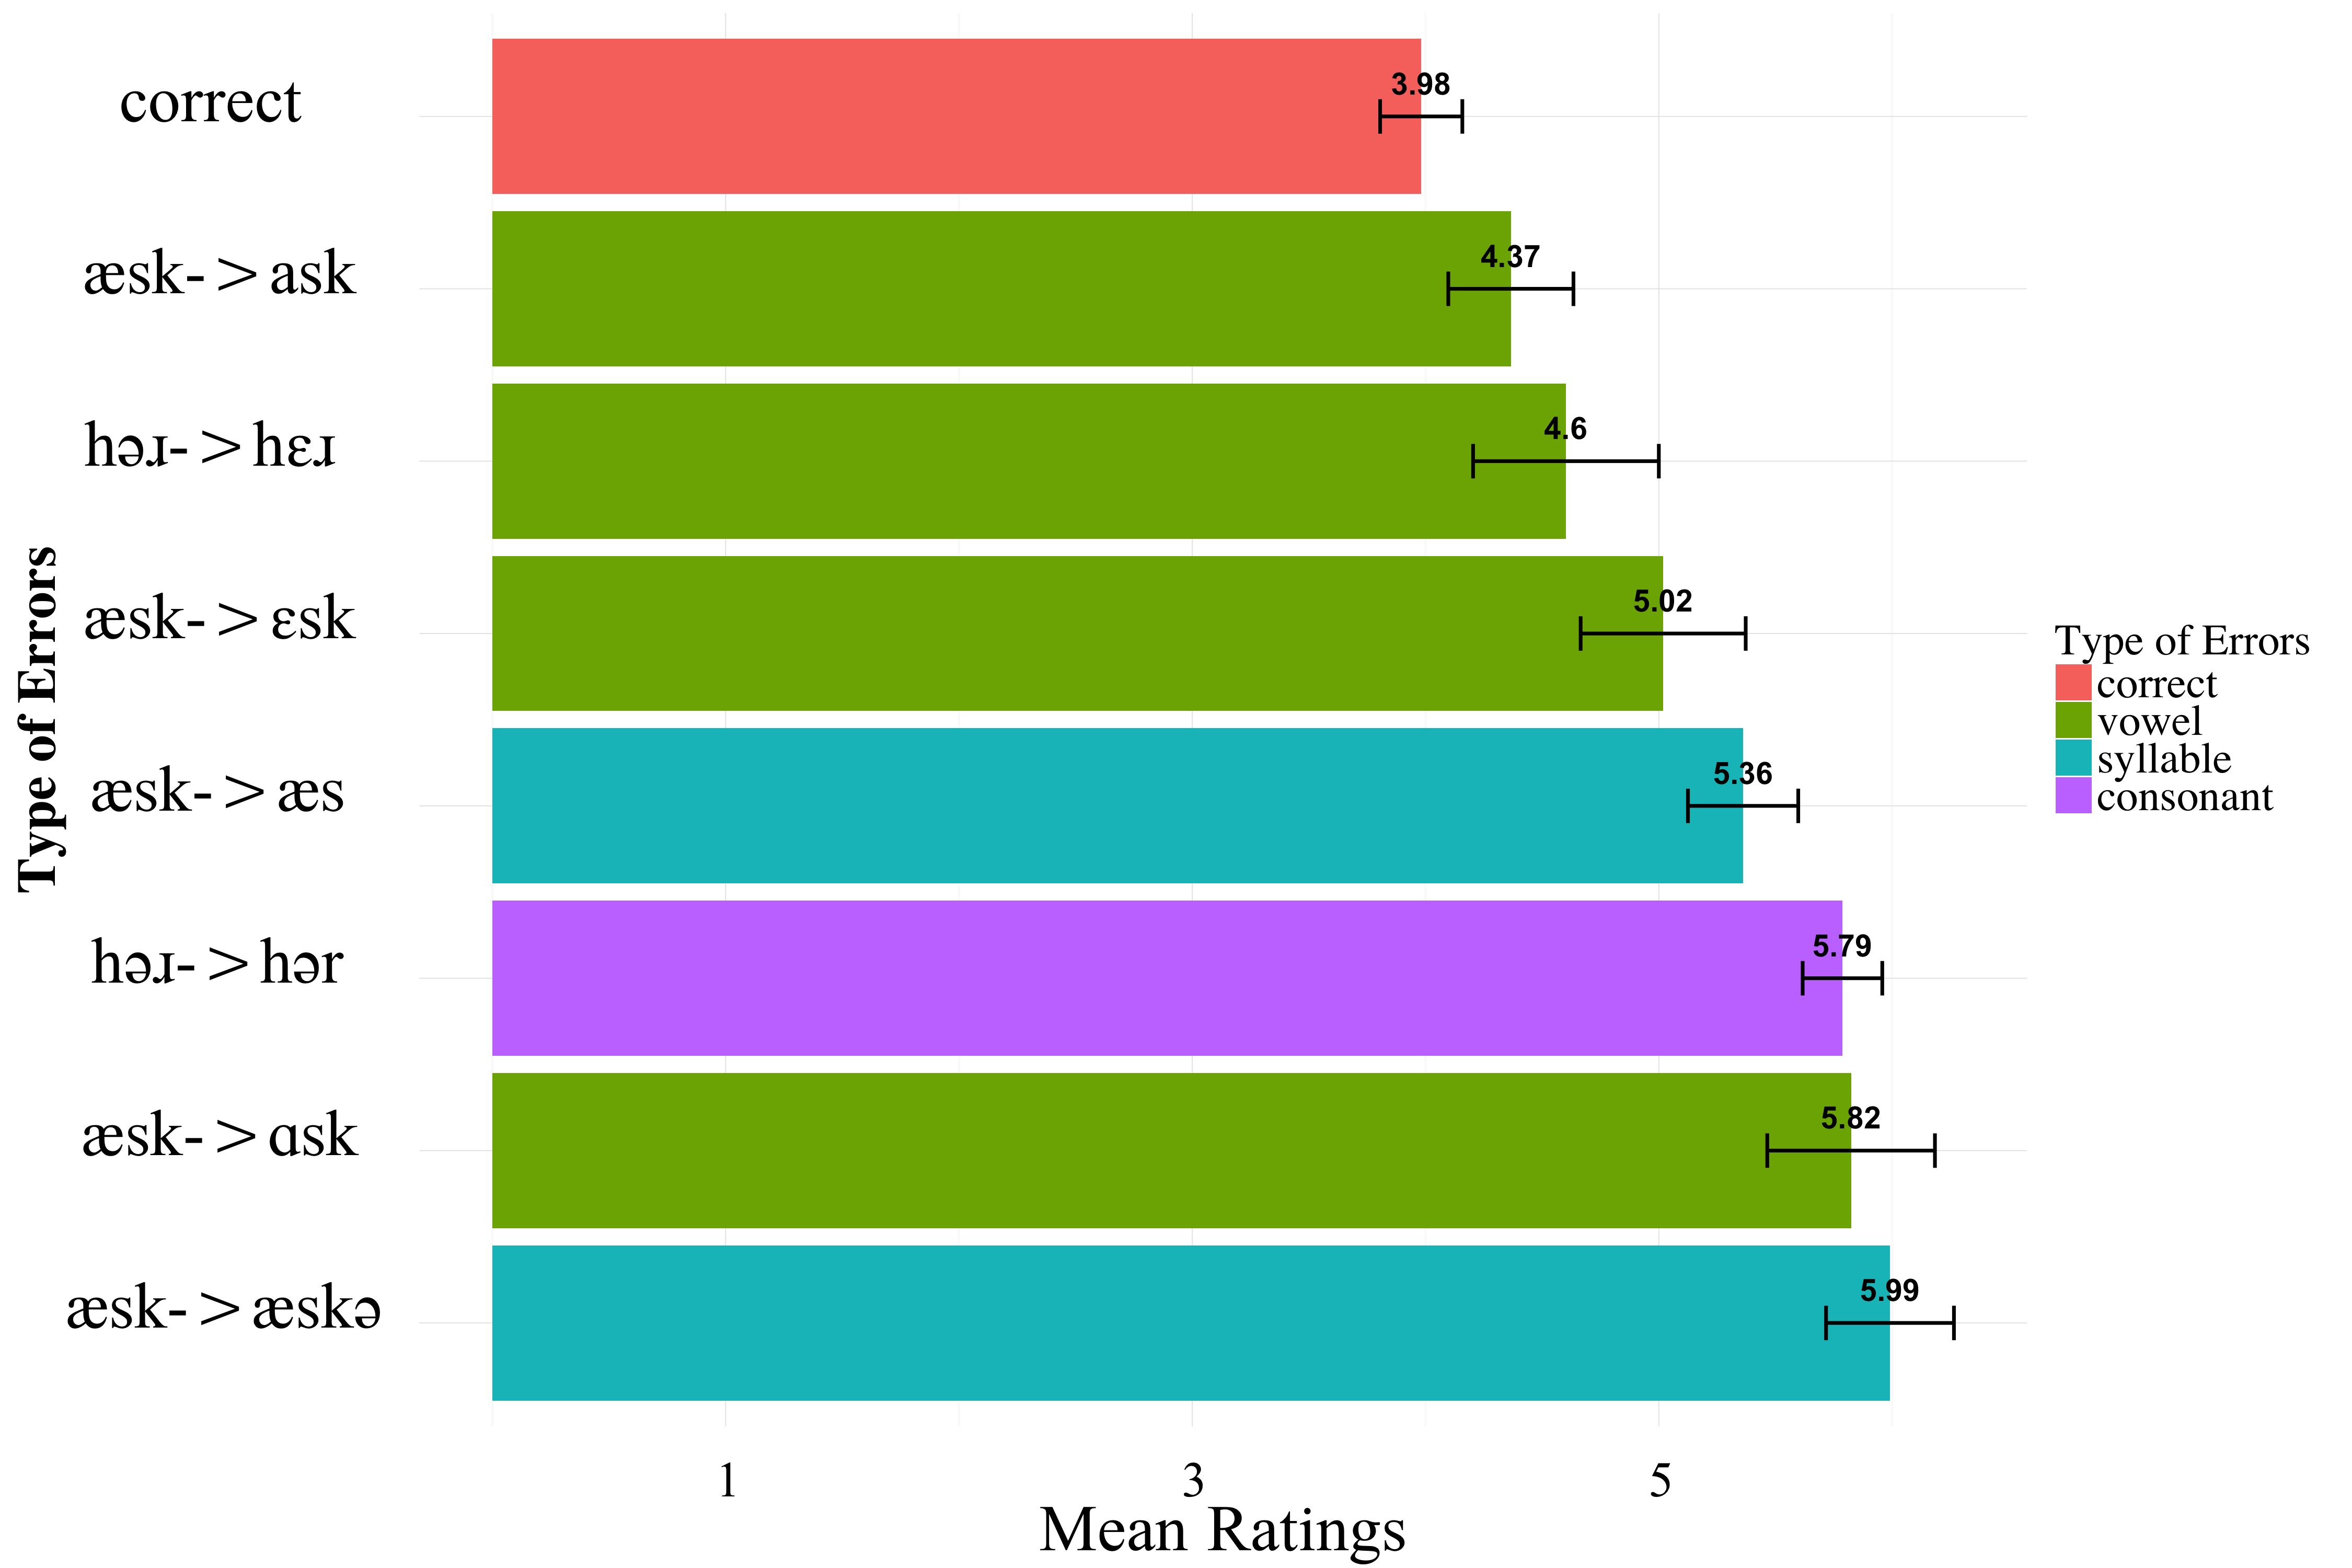
\includegraphics[width=0.8\linewidth]{ak_detailed}
\end{figure}
\end{block}}
\only <2>{
\begin{block}{Gao (2016):The trend does not always hold}
\begin{figure}
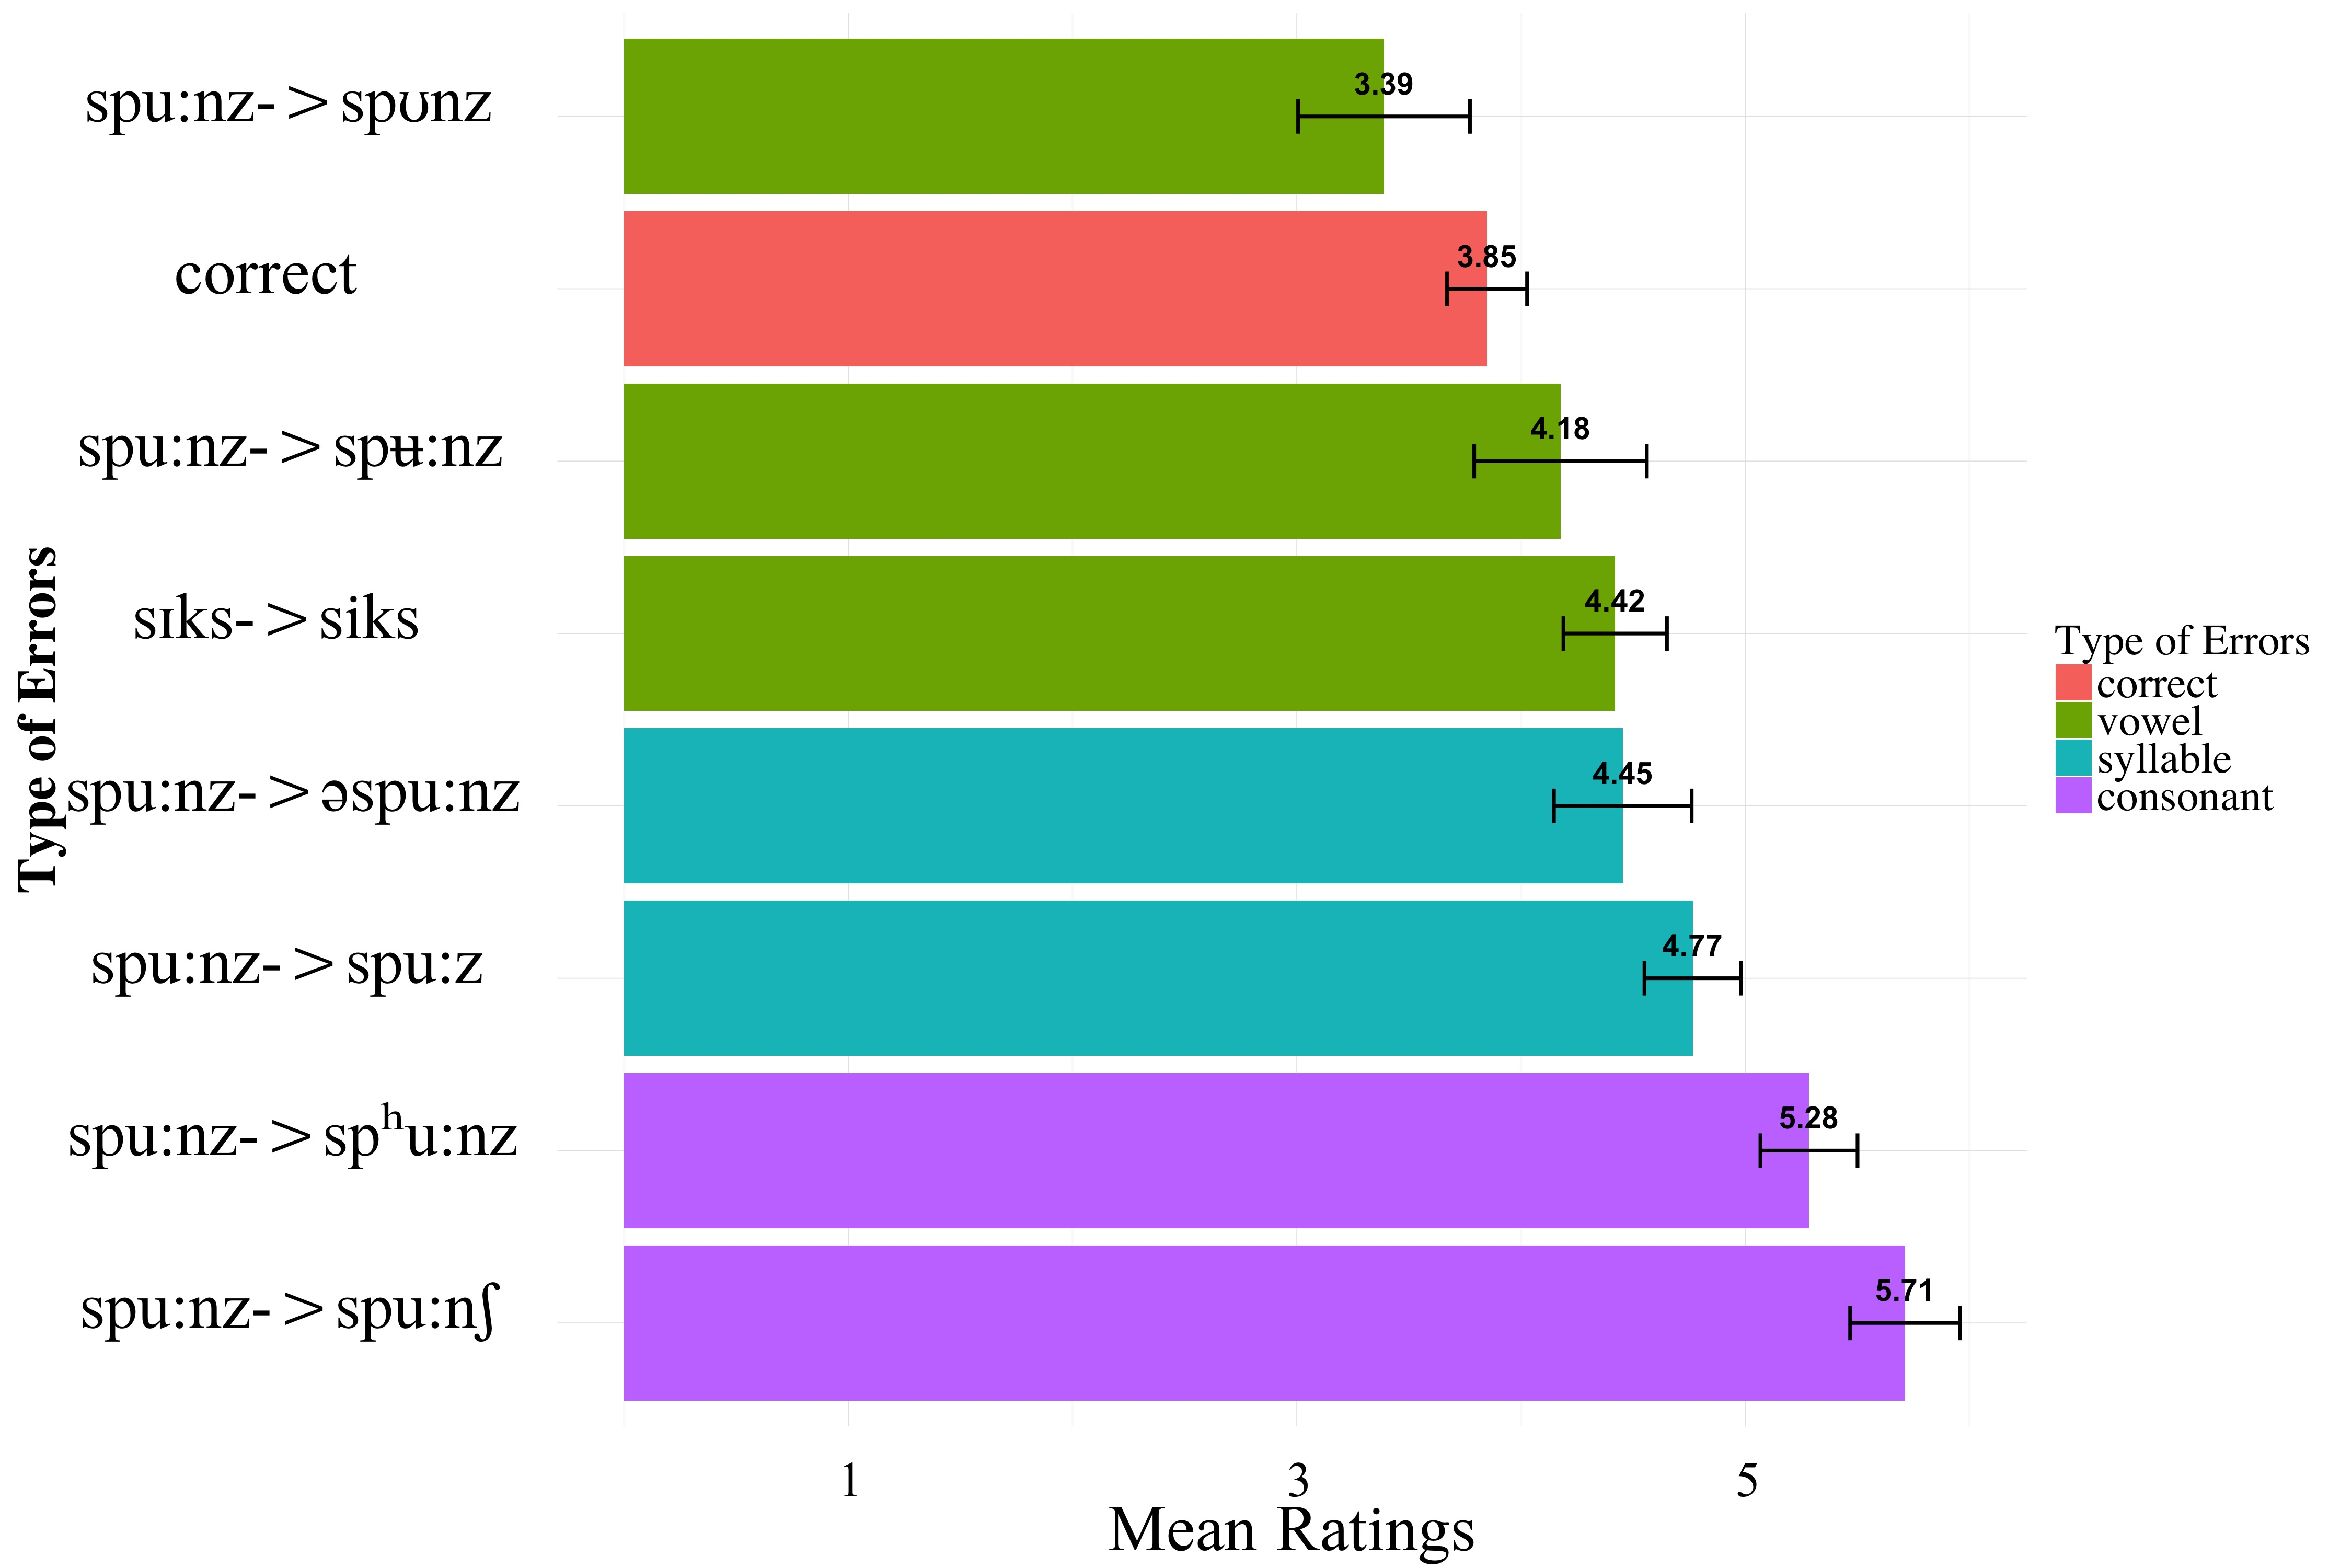
\includegraphics[width=0.8\linewidth]{ss_detailed}
\end{figure}
\end{block}}
\only <3>{
\begin{block}{Gao (2016):The trend does not always hold}
\begin{figure}
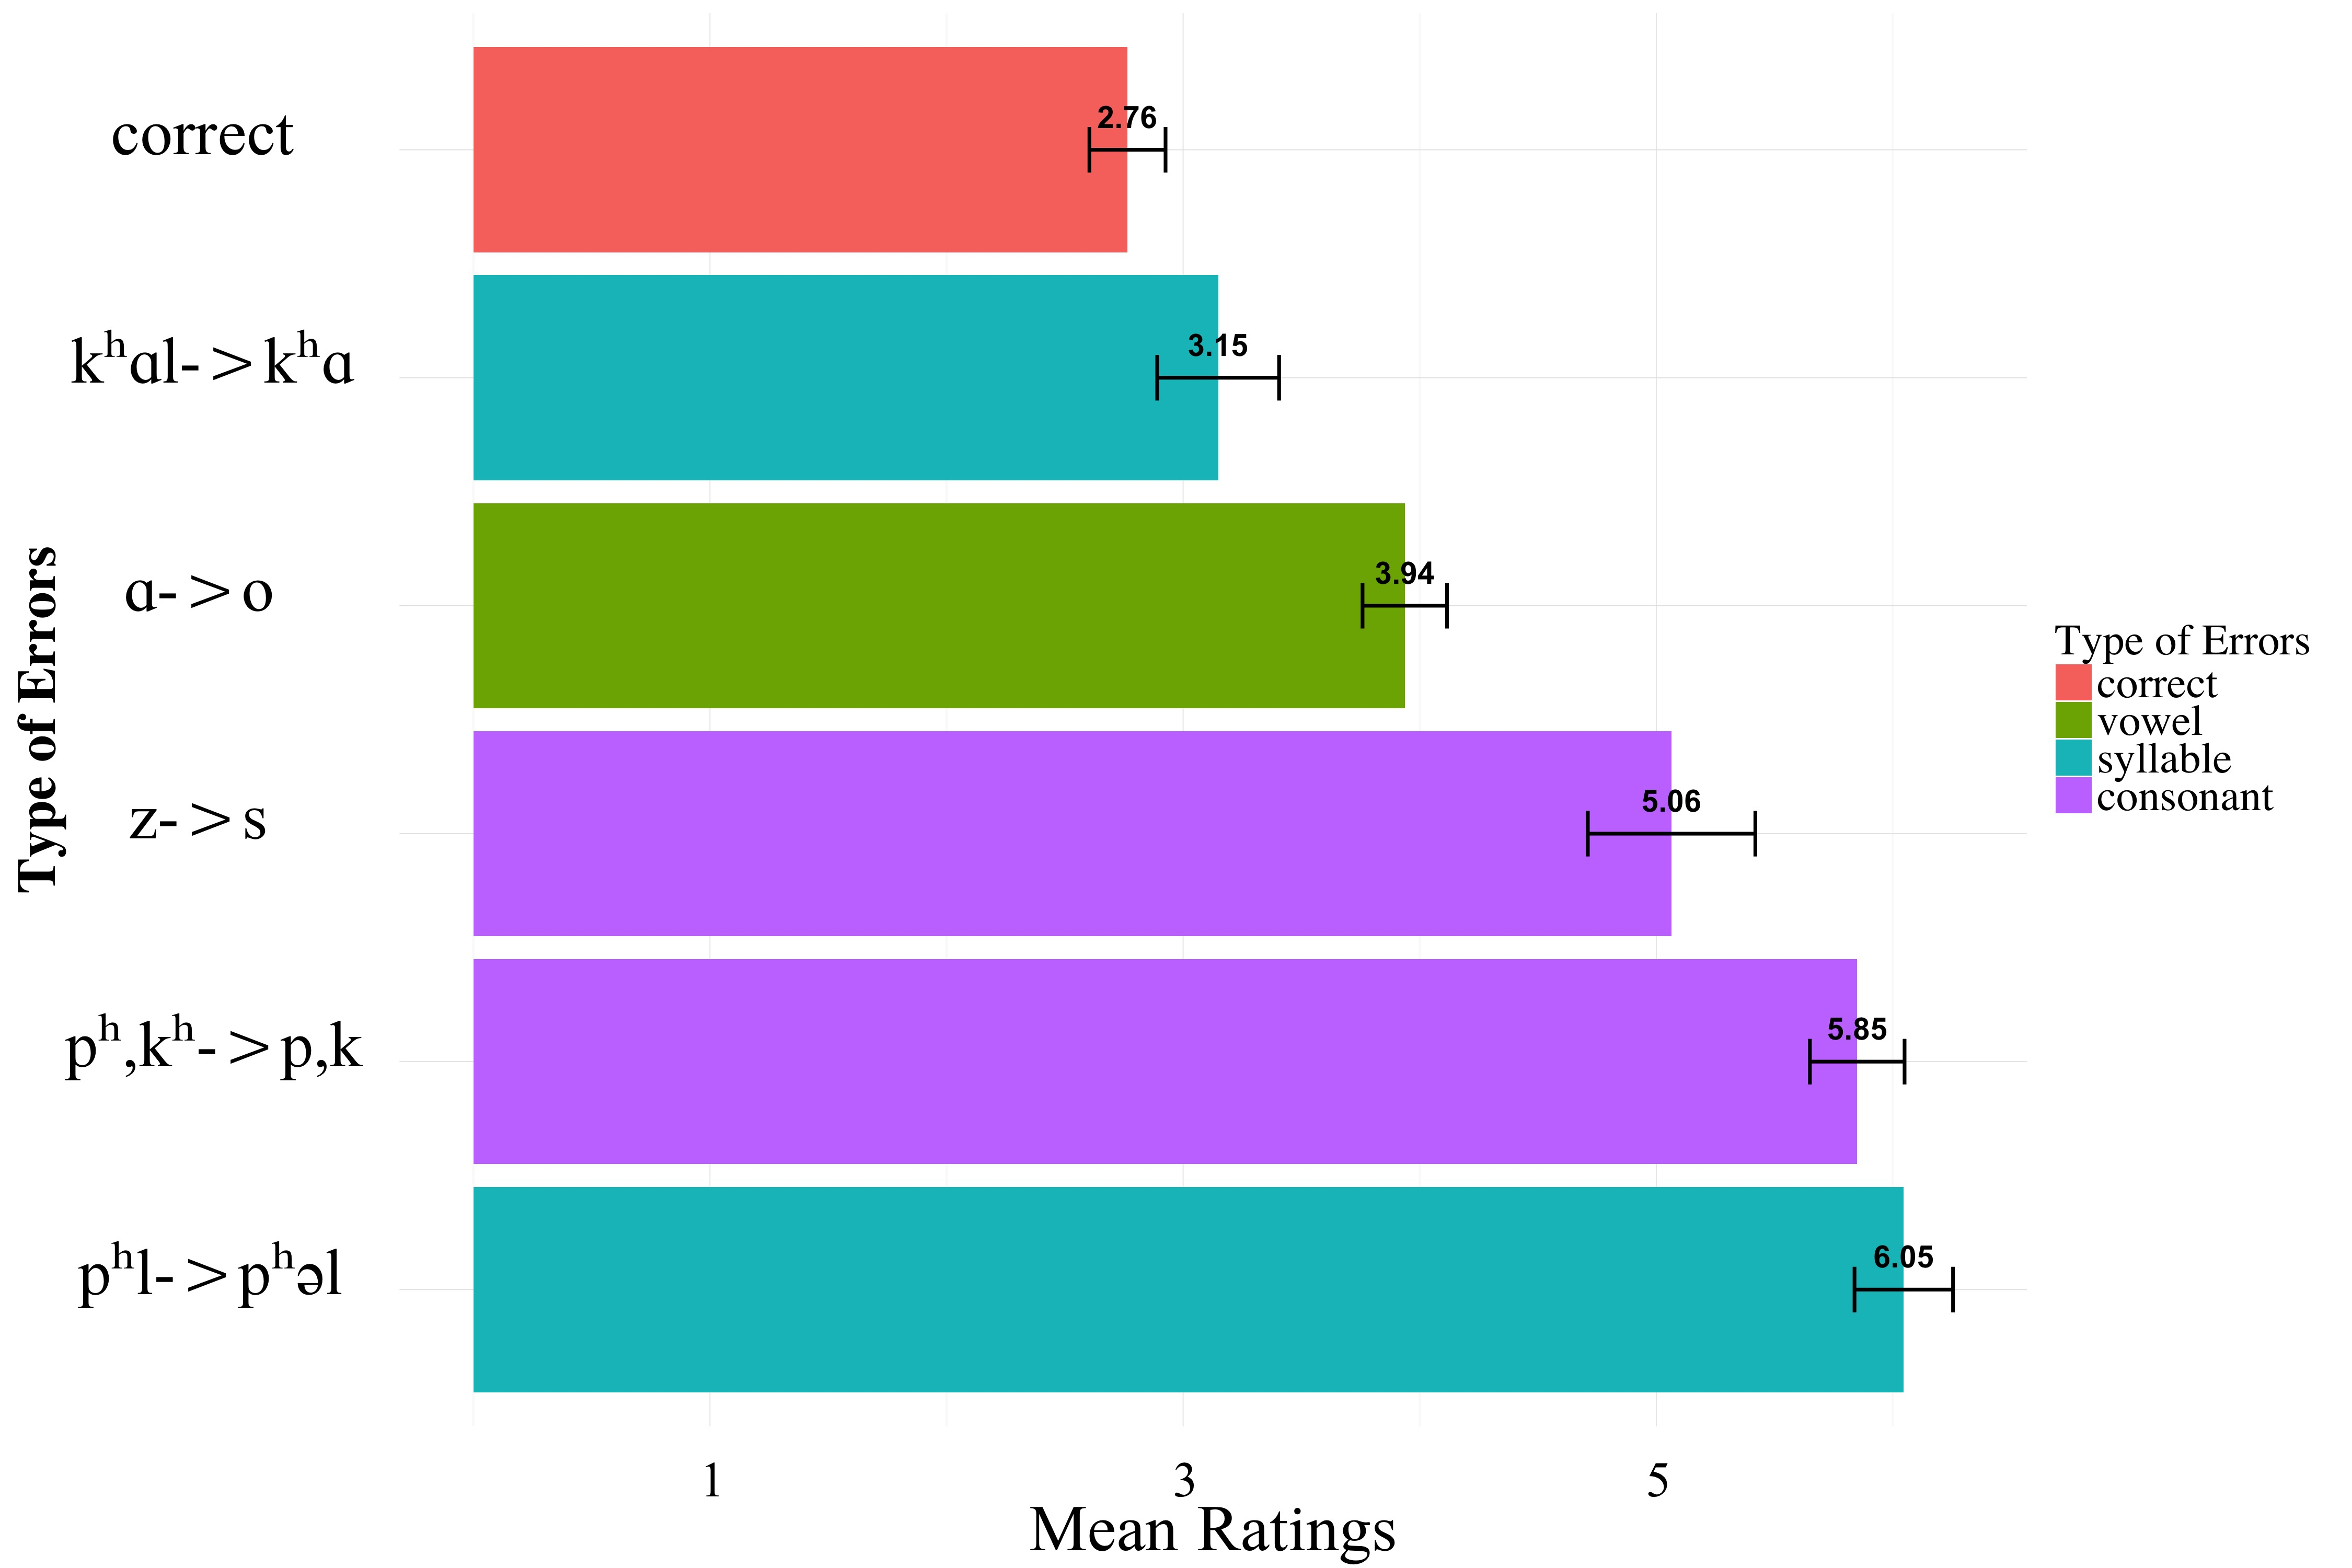
\includegraphics[width=0.8\linewidth]{pc_detailed}
\end{figure}
\end{block}}
\only <4>{
\begin{block}{Gao (2016):The trend does not always hold}
\begin{figure}
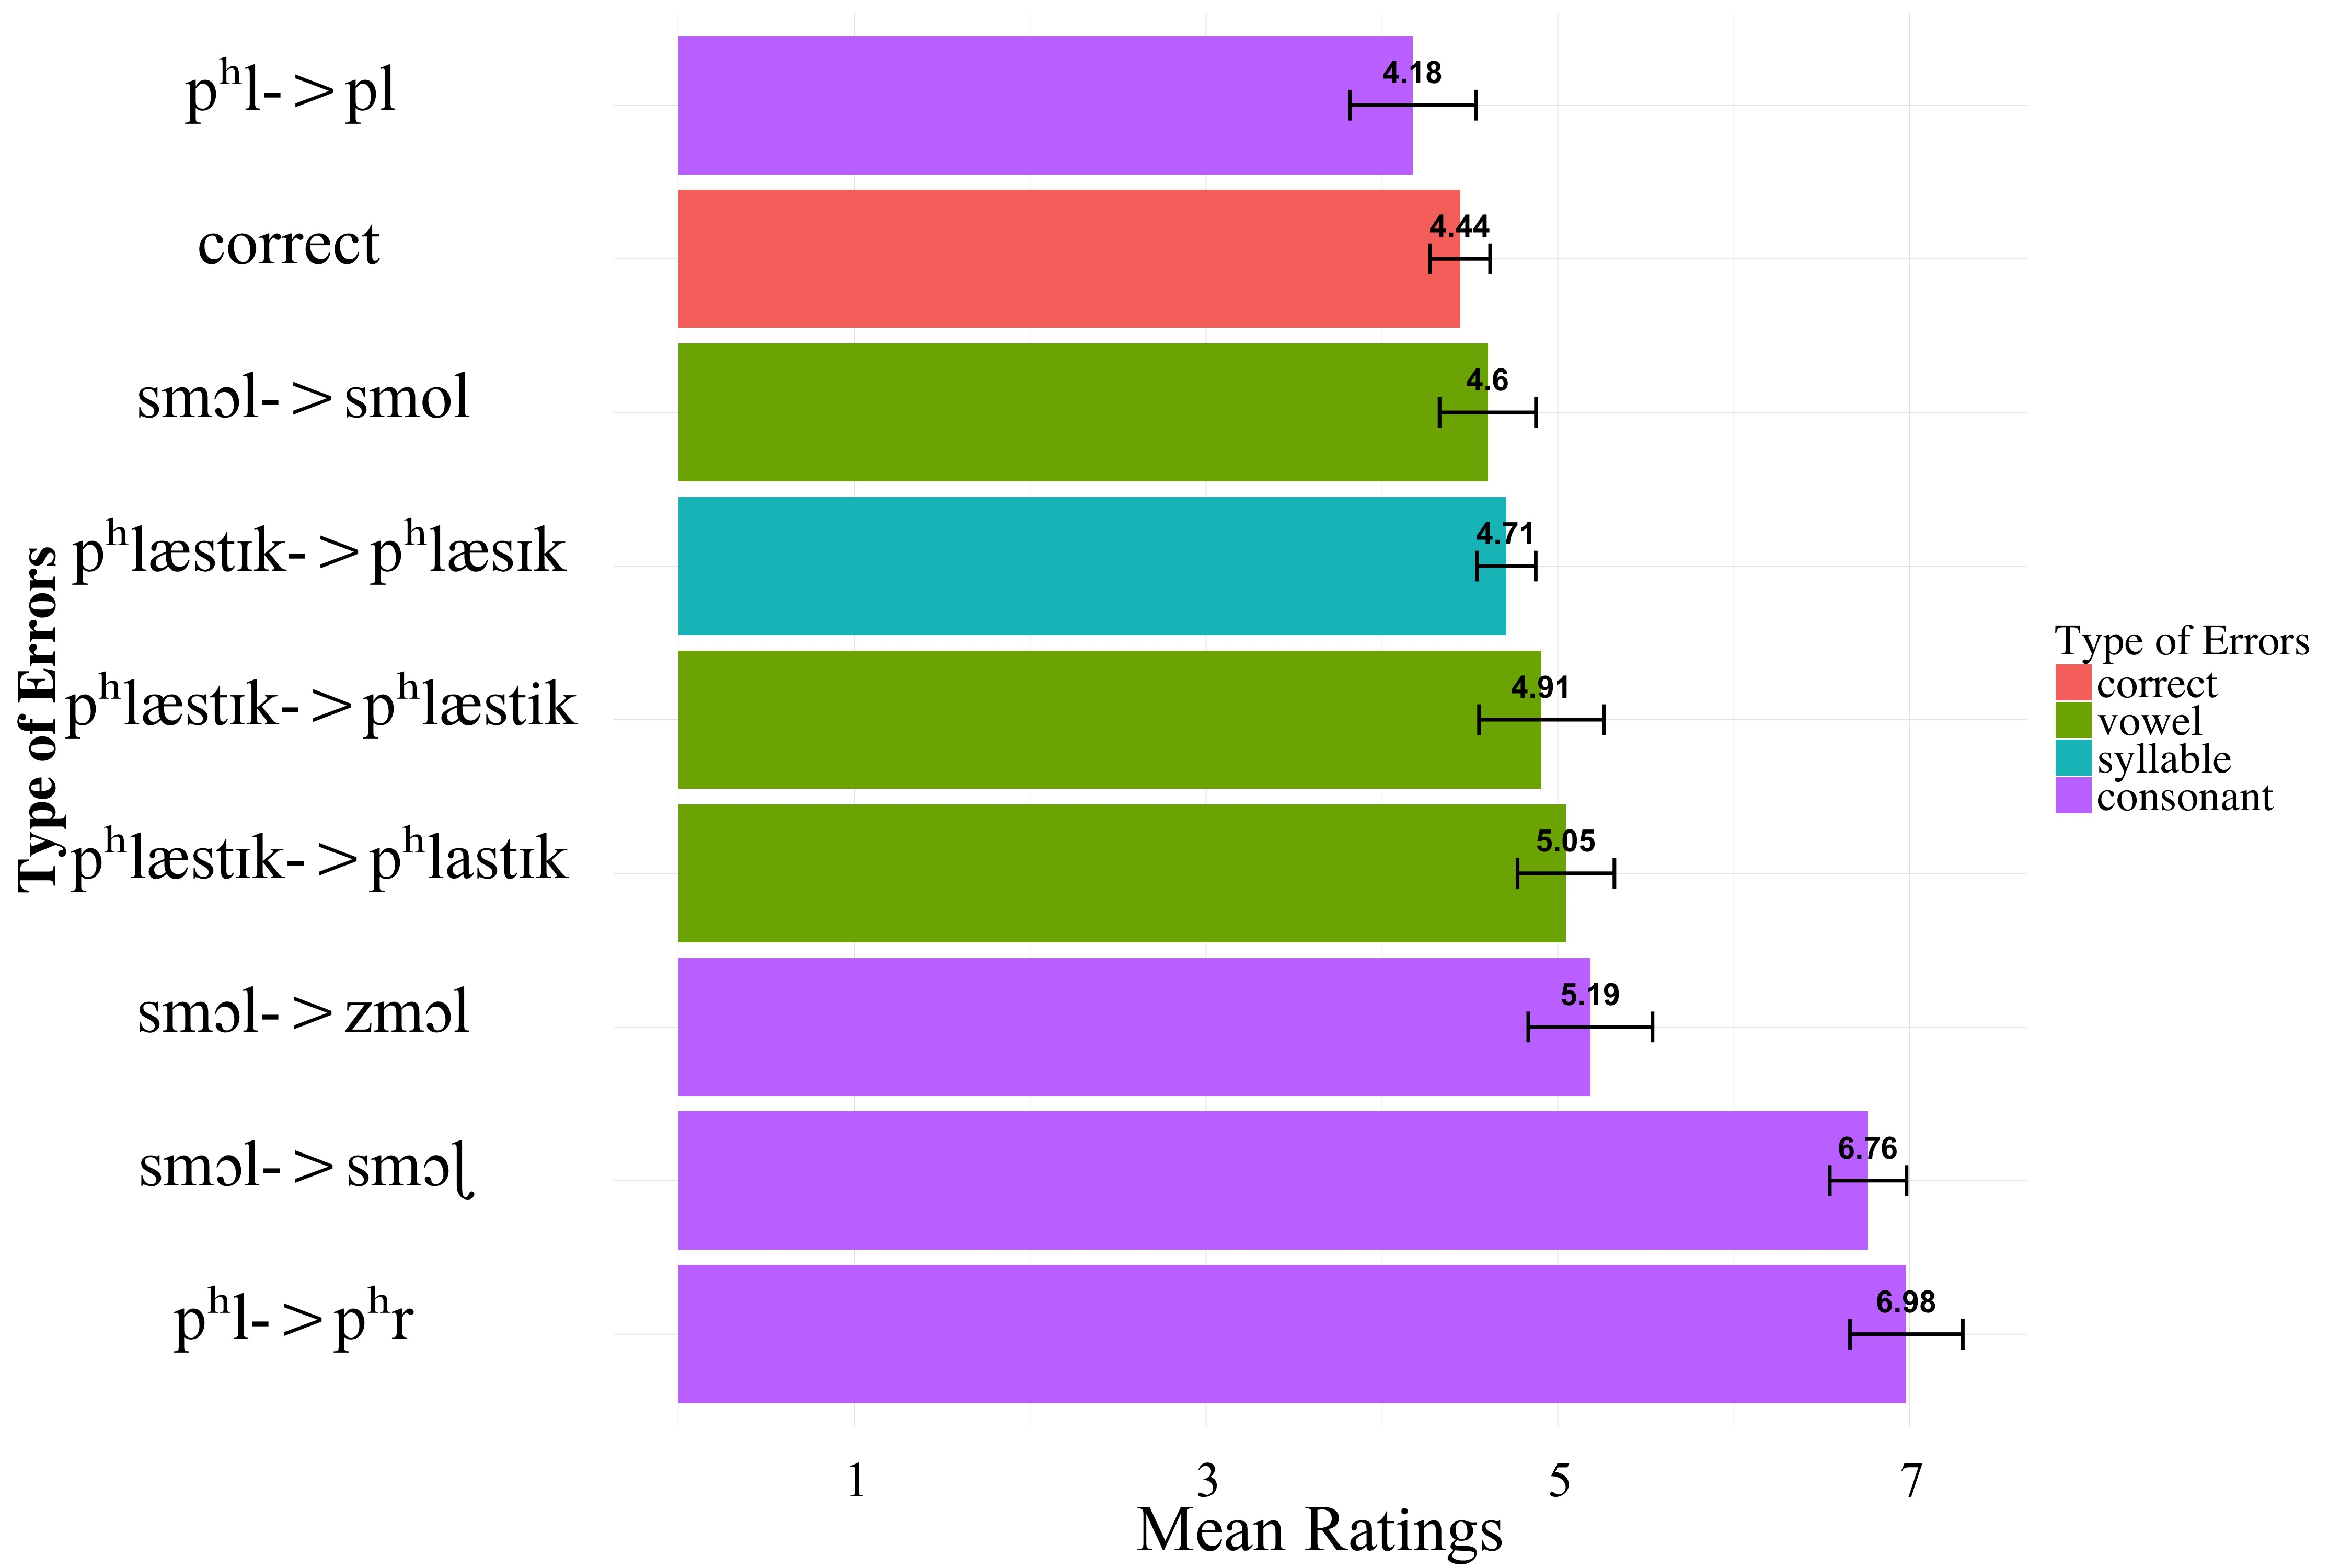
\includegraphics[width=0.8\linewidth]{sp_detailed}
\end{figure}
\end{block}}
\end{frame}
%--------------------
\subsection{Choropleth Map}
\begin{frame}
\frametitle{Supplemental materials \Romannum{2}:Ratings by State }
\begin{figure}
\includegraphics[width=0.9\linewidth]{heat}
\end{figure}
\end{frame}
%-----------------
\subsection{MaxEnt Constraints}
\begin{frame}
\frametitle{Supplemental materials \Romannum{3}:MaxEnt Constraints}
\begin{table}[]
\begin{tabular}{ll}
*{[}-sonorant,+continuant,+voice,+distributed{]}                  & 2.277 \\
*{[}+nasal,+DORSAL{]}                                             & 2.489 \\
*{[}-anterior,-distributed{]}                                     & 4.448 \\
*{[}-sonorant,-back{]}                                            & 3.986 \\
*{[}+voice{]}{[}-approximant{]}                                   & 0.349 \\
*{[}-word\_boundary{]}{[}+delayedRelease{]}                       & 4.571 \\
*{[}-CORONAL{]}{[}-approximant{]}                                 & 5.217 \\
*{[}-continuant{]}{[}-approximant{]}                              & 2.355 \\
*{[}-word\_boundary{]}{[}-sonorant,+voice{]}                      & 2.312 \\
*{[}+distributed{]}{[}+consonantal{]}                             & 2.15  \\
*{[}+continuant,+voice{]}{[}-word\_boundary{]}                    & 2.229 \\
*{[}+distributed{]}{[}-CORONAL{]}                                 & 0.921 \\
*{[}+sonorant{]}{[}-word\_boundary{]}                             & 5.019 \\
*{[}+LABIAL{]}{[}-CORONAL{]}                                      & 4.001 \\
\vdots & \vdots \\
\end{tabular}
\end{table}
\end{frame}

\end{document}